\documentclass{article}
\linespread{1.3}
\usepackage[margin=50pt]{geometry}
\usepackage{amsmath, amsthm, amssymb, amsthm, tikz, fancyhdr, float, graphicx, spverbatim, systeme}
\pagestyle{fancy}
\renewcommand{\headrulewidth}{0pt}
\newcommand{\changefont}{\fontsize{15}{15}\selectfont}

\fancypagestyle{firstpageheader}{
  \fancyhead[R]{
    \changefont
    \parbox[t]{4cm}{ % Adjust width as needed
      Michael Huang\\
      EN.625.740.81\\
      Homework 2
    }
  }
}

\begin{document}

\thispagestyle{firstpageheader}
{\Large 

\section*{1.}
Let \(X\) have an exponential distribution
\[
  p(x|v) = 
  \begin{cases}
    v e^{-v x}, & x \geq 0 \\
    0, & \text{otherwise.}
  \end{cases}
\]

\subsection*{(a)} 
Sketch \(p(x|v)\) versus \(x\) for a fixed value of the parameter \(v\).
\begin{figure}[h!]
  \centering
  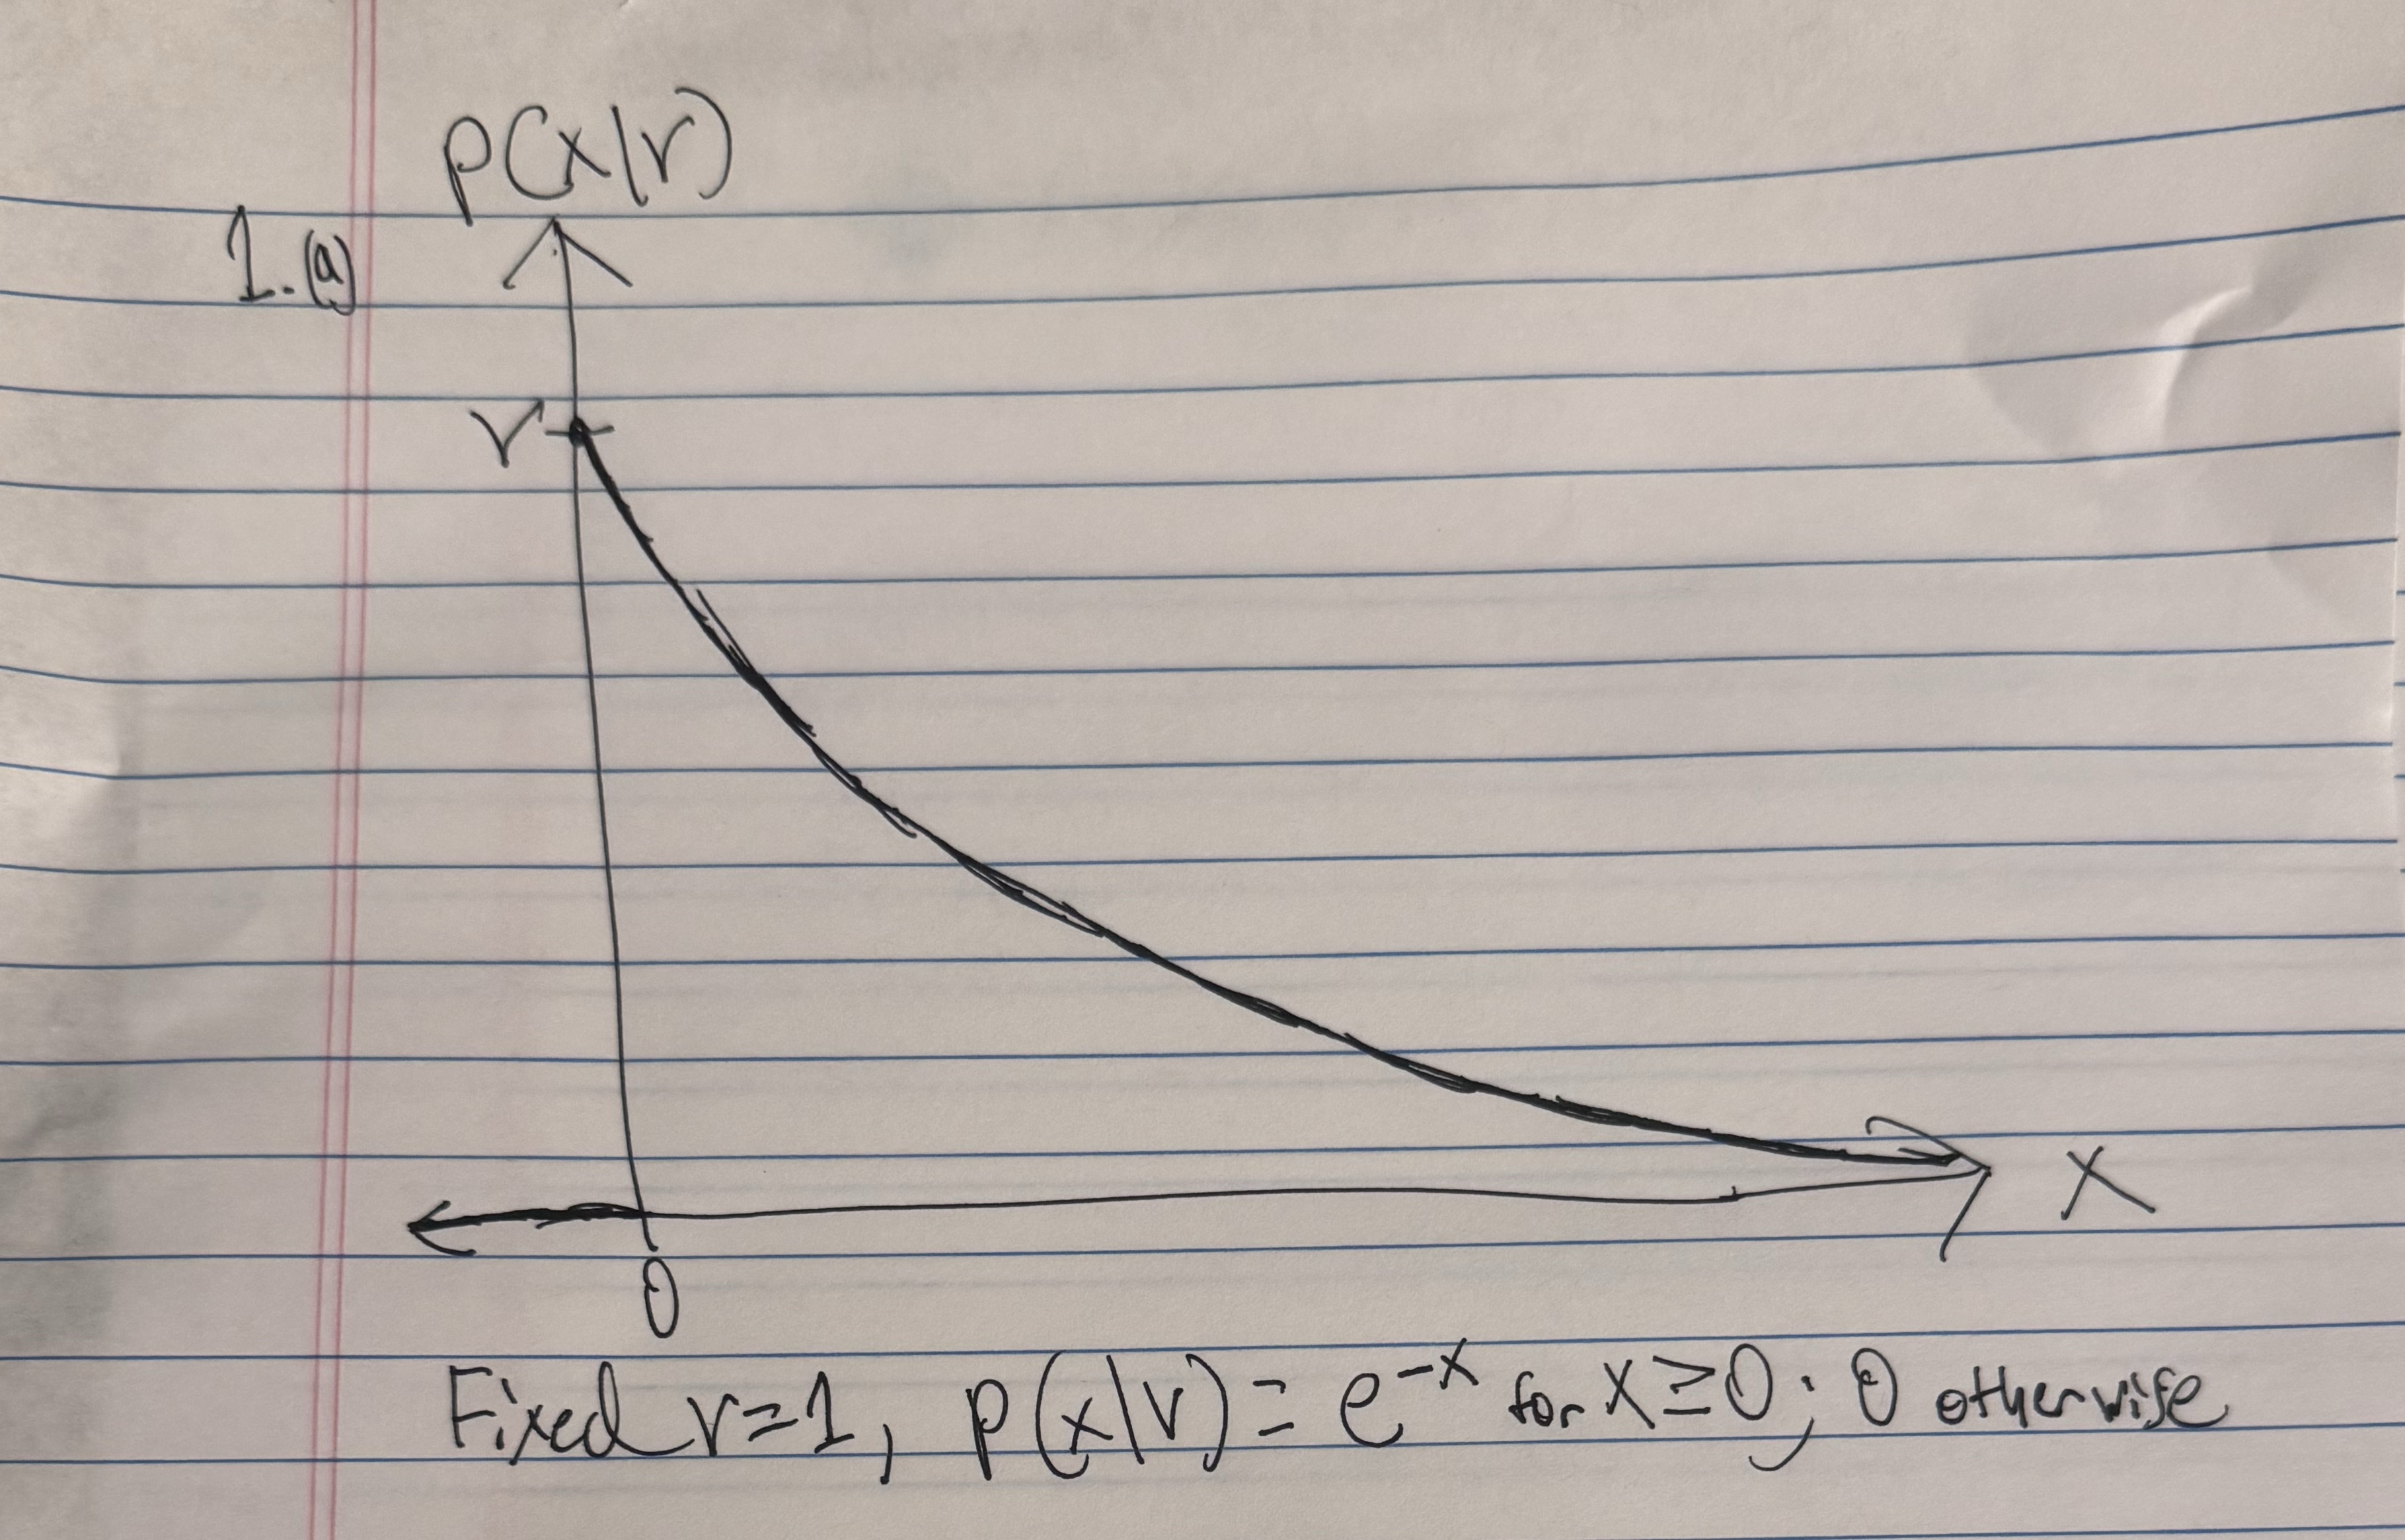
\includegraphics[width=400pt]{1a_graph.png}
\end{figure} 

\subsection*{(b)}
Sketch \(p(x|v)\) versus \(v\), \(v > 0\) for a fixed value of \(x\).
\begin{figure}[h!]
  \centering
  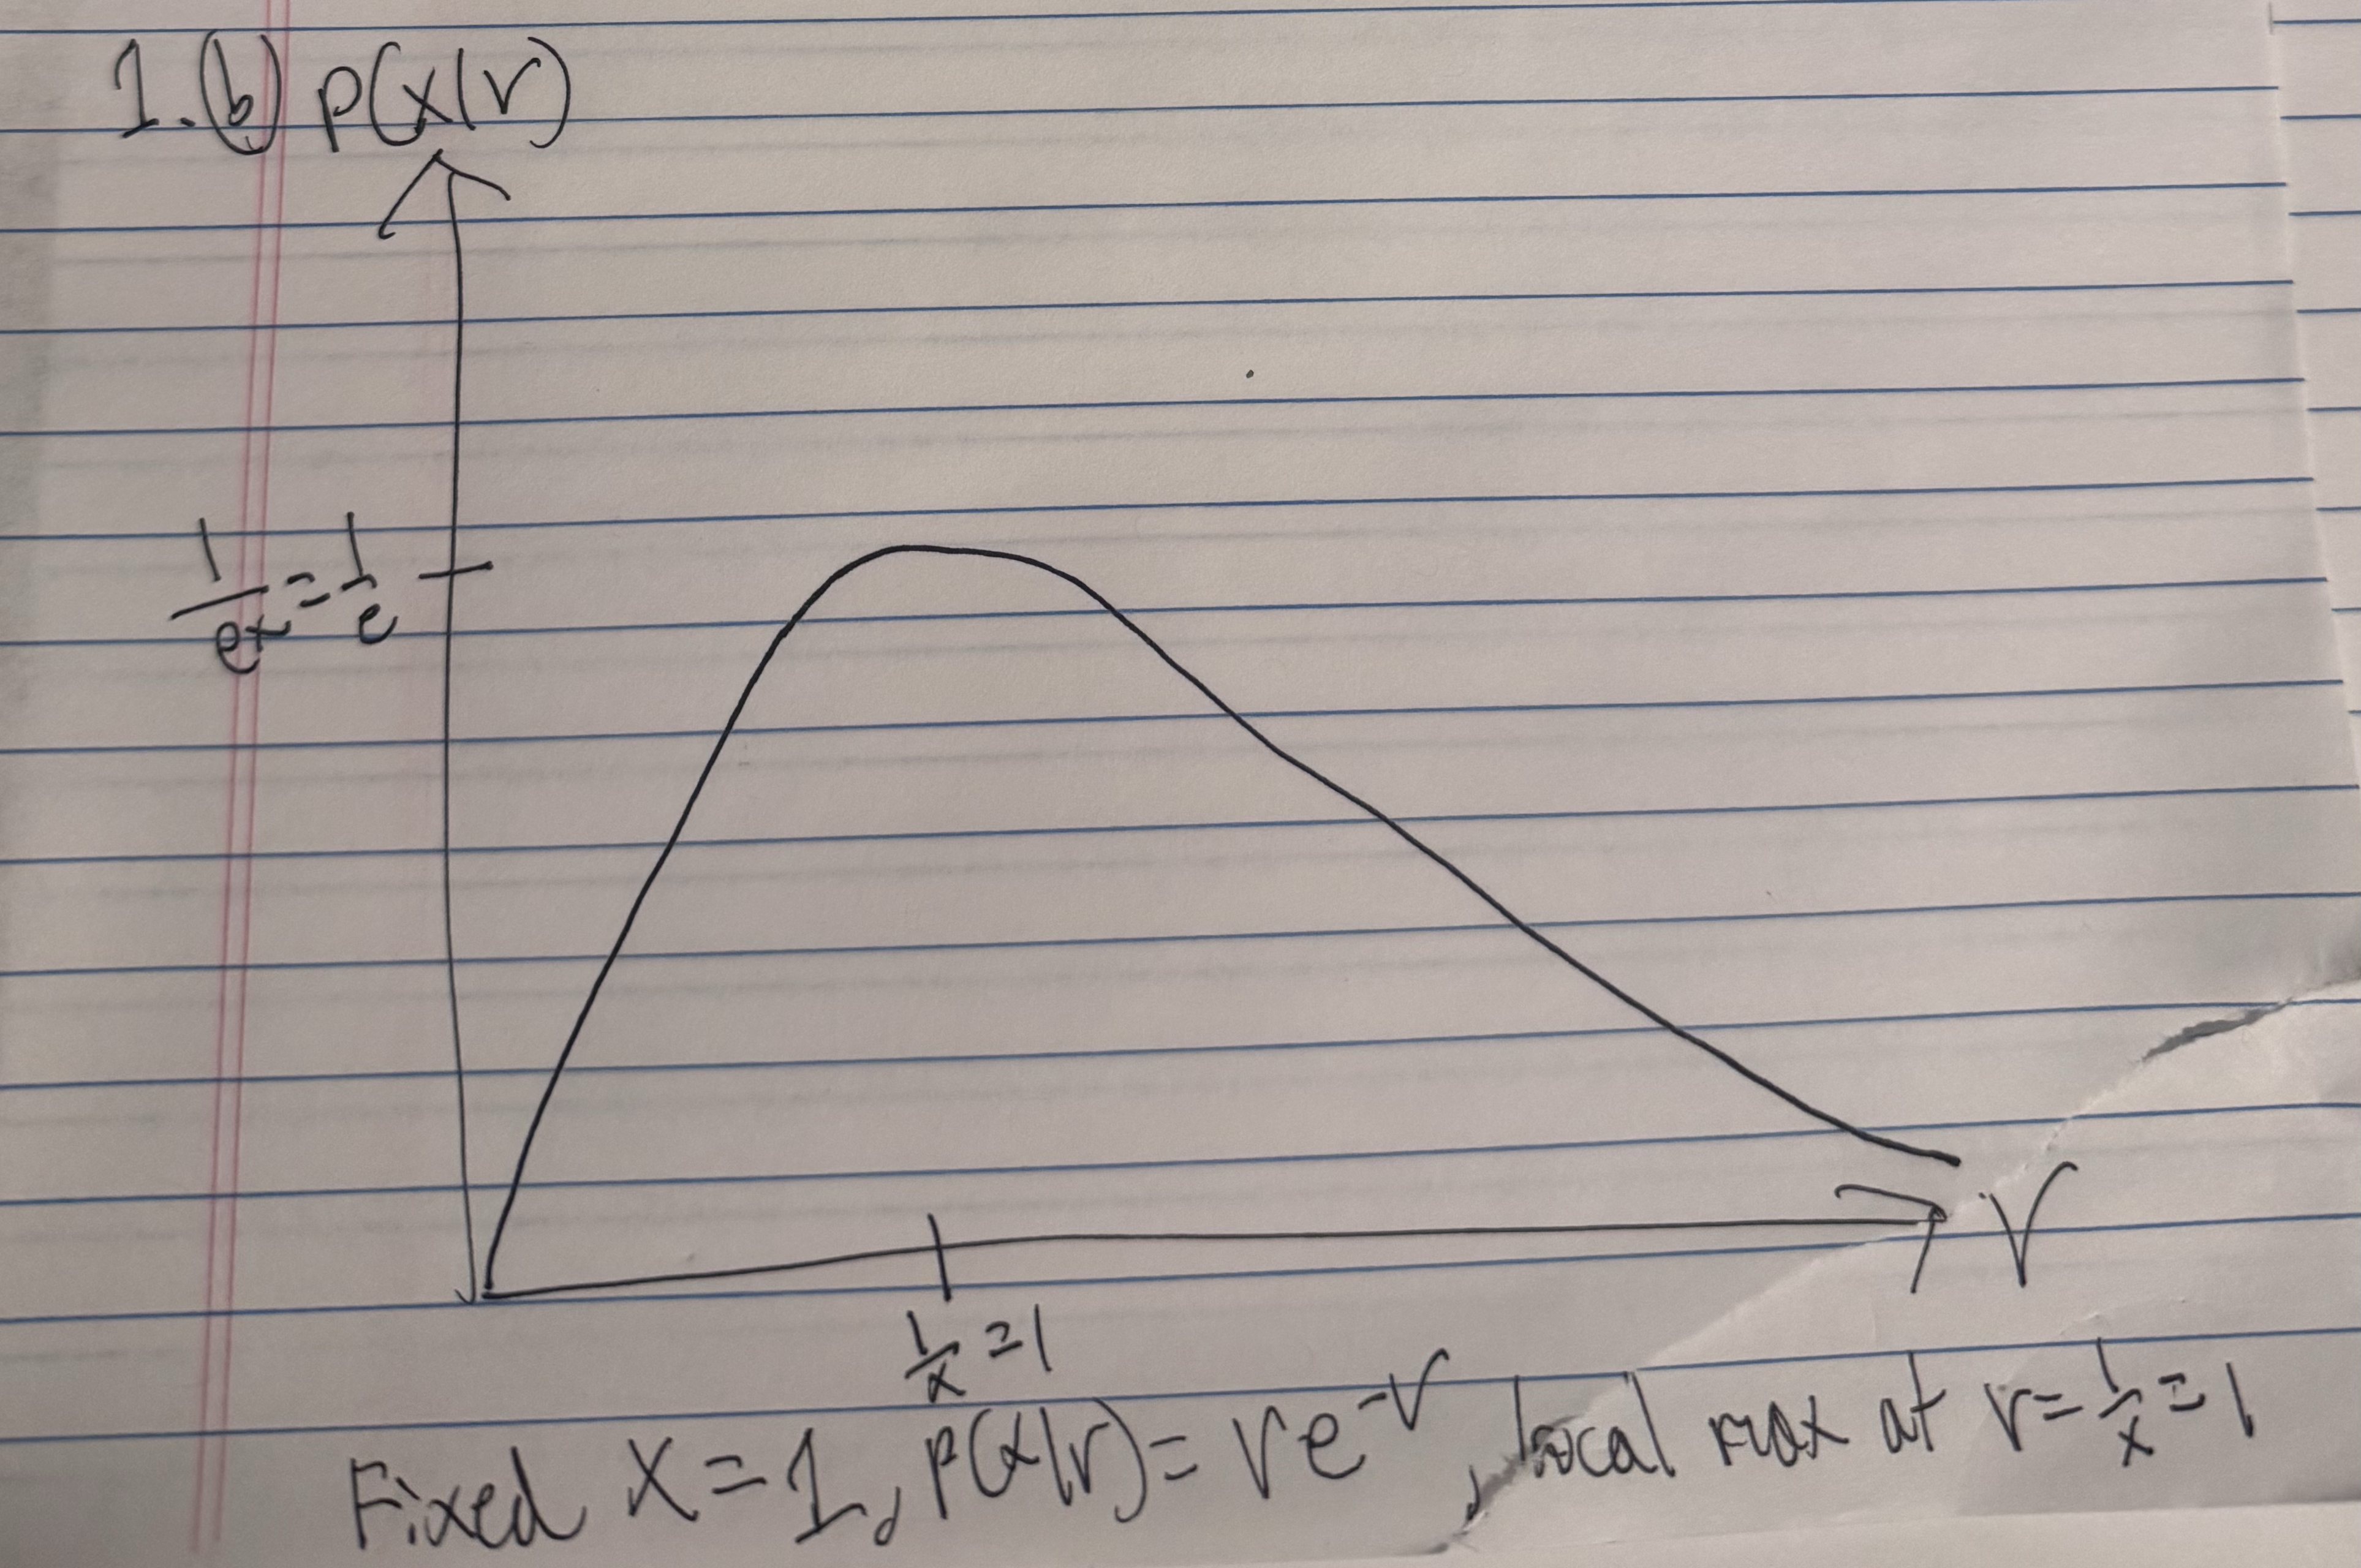
\includegraphics[width=400pt]{1b_graph.png}
\end{figure}  \\ \\ \\ \\ \\ \\ 

\subsection*{(c)}
Suppose that \(n\) samples \(x_1, \dots, x_n\) are drawn independently according to \(p(x|v)\). Show that the maximum likelihood estimate for \(v\) is given by 
\[
  \hat{v} = \frac{1}{\frac{1}{n} \sum_{k=1}^n x_k}
\]
We can derive the MLE for \(v\) directly. We first write the likelihood function. Suppose \(x_1, \dots, x_n\) are independent observations drawn from the exponential distribution, as defined by \(p(x|v)\); we just multiply for a likelihood function of 
\[
  L(v) = \prod_{k=1}^{n} v e^{-vx_k}
\]
We then take the log likelihood:
\[
  l(v) = \ln(\prod_{k=1}^{n} v e^{-vx_k})
\]
\[
  = \sum_{k=1}^{n} \ln(v e^{-vx_k})
\]
\[
  = \sum_{k=1}^{n} (\ln(v) + \ln(e^{-vx_k}))
\]
\[
  = \sum_{k=1}^{n} (\ln(v) - vx_k)
\]
\[
  = n\ln(v) - \sum_{k=1}^{n} vx_k
\]
and differentiate:
\[
  \frac{dl}{dv} = \frac{d}{dv} (n\ln(v) - \sum_{k=1}^{n} vx_k)
\]
\[
  = \frac{n}{v} - \sum_{k=1}^{n} x_k
\]
Verifying this is a maximum by taking the second derivative:
\[
  \frac{d^2l}{dv^2} = \frac{d}{dv} (\frac{n}{v} - \sum_{k=1}^{n} x_k) 
\]
\[
  = -\frac{n}{v^2} - 0 = -\frac{n}{v^2}
\]
which we see is indeed negative as both the numerator \(n > 0\) and the denominator is also always positive; multiplying by this then gives us a negative value, so this is indeed a maximum.
Finally, set equal to zero to solve:
\[
  0 = \frac{n}{v} - \sum_{k=1}^{n} x_k
\]
\[
  \sum_{k=1}^{n} x_k = \frac{n}{v}
\]
\[
  v = \frac{n}{\sum_{k=1}^{n} x_k}
\]
So we get 
\[
  \hat{v} =  \frac{n}{\sum_{k=1}^{n} x_k} = \frac{1}{\frac{1}{n}\sum_{k=1}^{n} x_k}
\]
exactly as we sought to find.

}
{\Large 

\section*{2.}
Let \(X\) have a uniform distribution
\[
  p(x|v) = 
  \begin{cases}
    \frac{1}{v}, & 0 \leq x \leq v \\
    0, & \text{otherwise.}
  \end{cases}
\]

\subsection*{(a)} 
Sketch \(p(x|v)\) versus \(v\) for an arbitrary value of \(x\).
\begin{figure}[h!]
  \centering
  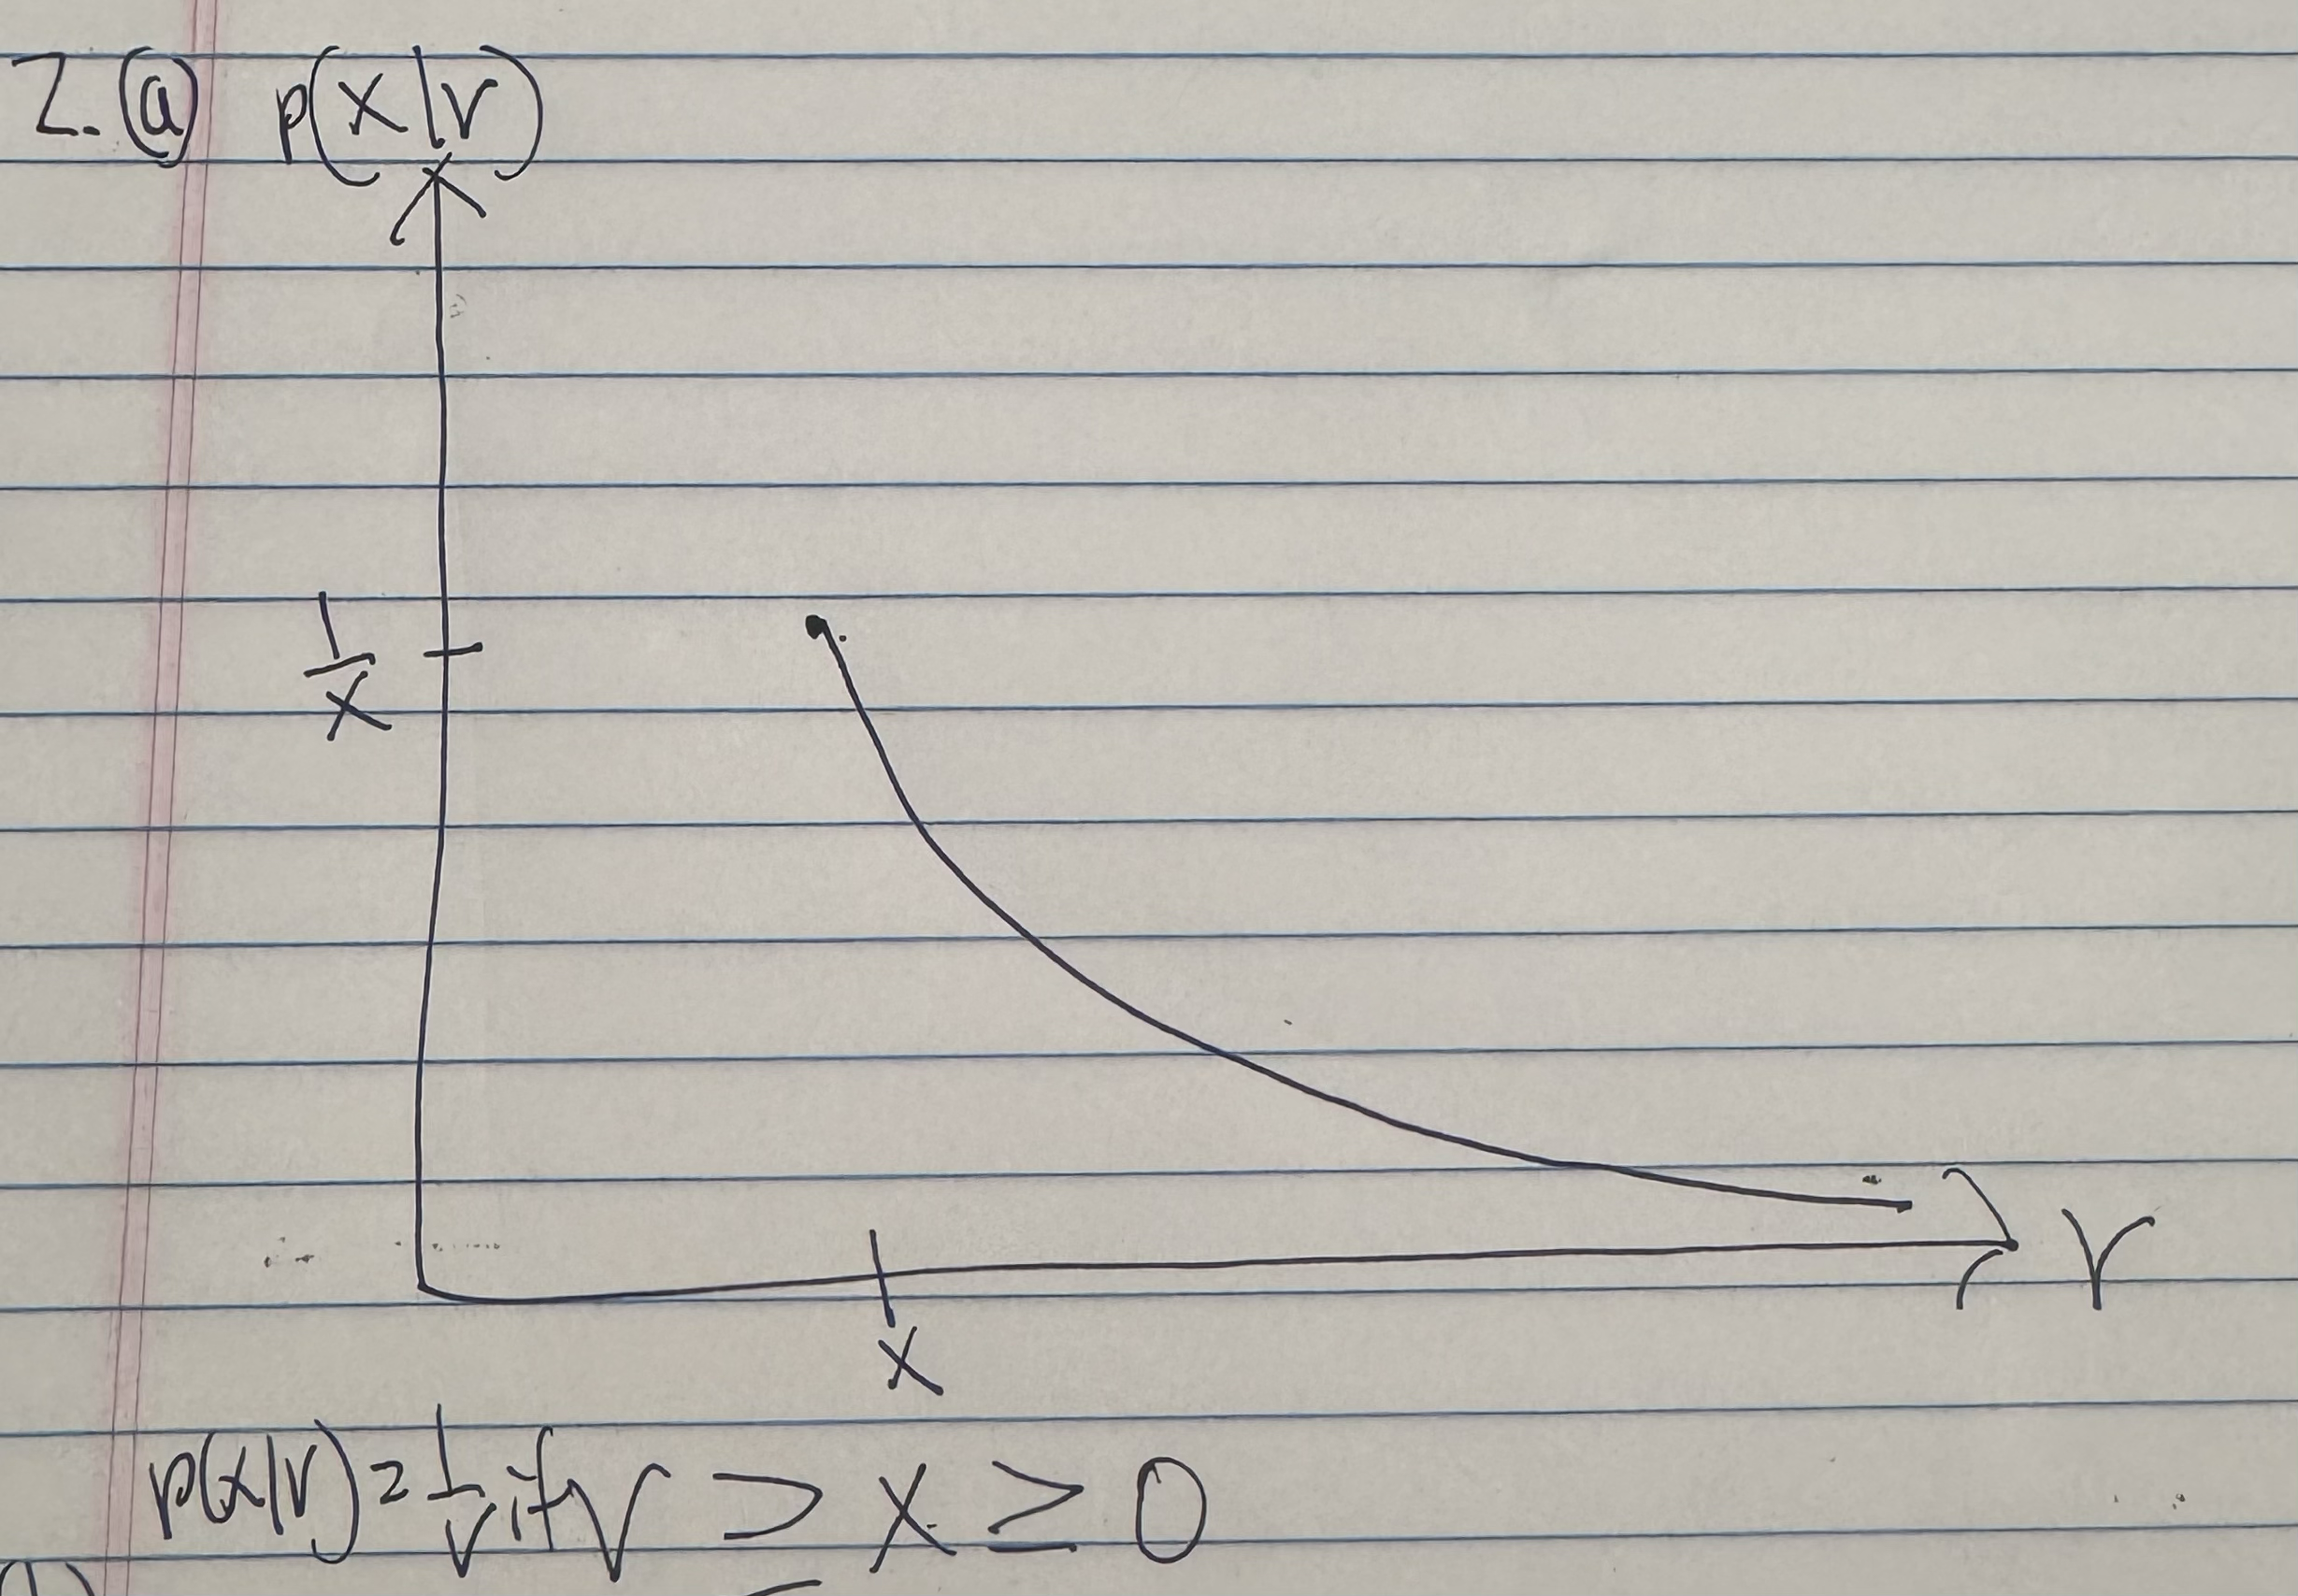
\includegraphics[width=400pt]{2a_graph.png}
\end{figure}

\subsection*{(b)}
Suppose that \(n\) samples \(x_1, \dots, x_n\) are drawn independently according to \(p(x|v)\). Show that the maximum likelihood estimate for \(v\) is \(\text{max}_k x_k\). \\ \\
By definition, we have that 
\[
  L(v) = \prod_{k=1}^{n} p(x_k|v) 
\]
\[
  L(v) = 
  \begin{cases}
    \frac{1}{v^n}, & v \geq \max_k(x_k) \\
    0, & \text{otherwise.}
  \end{cases}
\]
We note that \(\frac{1}{v^n}\) continuously decreases as \(v\) increases; we therefore must choose the smallest possible value of \(v\). We also have the restriction that \(v\) must be at least as large as the maximum \(x_k\) value, or \(\text{max}_k x_k\). We therefore have that 
\[
  \hat{v} = \max_kx_k 
\]
exactly as we sought to show.

\subsection*{(c)}
Find the method of moments estimator for \(v\). \\ \\
Let \(X_1, \dots, X_n \sim \text{Uniform}(0, v)\). We therefore have the first population moment as
\[
  \alpha_1 = E[X] = \int_{0}^{v} x \cdot \frac{1}{v} dx
\]
\[
  = \frac{1}{v} \cdot \frac{x^2}{2} |_{0}^{v}
\]
\[
  = \frac{1}{v} \cdot \frac{v^2}{2} - 0
\]
\[
  E[X] = \frac{v}{2}
\]
We would then also have the corresponding first sample moment as 
\[
  \hat{\alpha_1} = \frac{1}{n} \sum_{k=1}^{n} x_k = \bar{x}
\]
So we finally take the method of moments estimator to be 
\[
  \frac{\hat{v}}{2} = \bar{x}
\]
\[
  \boxed{\hat{v} = 2 \bar{x}}
\]

}
{\Large 

\section*{3.}
Let \(\mathbf{X}\) be a binary (0, 1) vector with multivariate Bernoulli distribution
\[
  p(\mathbf{x}|\mathbf{v}) = \prod_{i=1}^d v_i^{x_i} (1 - v_i)^{1-x_i}
\]
where \(\mathbf{v} = (v_1, \dots, v_d)^T\) is an unknown parameter vector, \(v_i\) being the probability that \(x_i = 1\). Show that the maximum likelihood estimate for \(\mathbf{v}\) is
\[
  \hat{\mathbf{v}} = \frac{1}{n} \sum_{k=1}^{n} \mathbf{x}_k
\]
We first evaluate the likelihood function, taking the product of all observations given \(n\) independent observations of \(\mathbf{x}\):
\[
  L(\mathbf{v}) = \prod_{k=1}^{n} p(\mathbf{x}_k | \mathbf{v}) = \prod_{k=1}^{n} \prod_{i=1}^d v_i^{x_{ki}} (1 - v_i)^{1-x_{ki}}
\]
We then take the log likelihood:
\[
  l(\mathbf{v}) = \log(\prod_{k=1}^{n} \prod_{i=1}^d v_i^{x_{ki}} (1 - v_i)^{1-x_{ki}})
\]
\[
  = \sum_{k=1}^{n} \sum_{i=1}^{d} \log(v_i^{x_{ki}} (1 - v_i)^{1-x_{ki}})
\]
\[
  l(\mathbf{v})= \sum_{k=1}^{n} \sum_{i=1}^{d} (x_{ki}\log(v_i) + (1 - x_{ki})\log(1-v_i))
\]
Now taking the derivative of this:
\[
  \frac{\partial l}{\partial v_i} = \frac{\partial}{\partial v_i}(\sum_{k=1}^{n} \sum_{i=1}^{d} (x_{ki}\log(v_i) + (1 - x_{ki})\log(1-v_i)))
\]
\[
  \frac{\partial l}{\partial v_i} = \sum_{k=1}^{n} \sum_{i=1}^{d} \frac{\partial}{\partial v_i} (x_{ki}\log(v_i) + (1 - x_{ki})\log(1-v_i))
\]
As we are only differentiating with respect to \(v_i\), everything within the inner sum becomes 0 except for the \(v_i\) term itself, so this essentially simplifies to 
\[
  \frac{\partial l}{\partial v_i} = \sum_{k=1}^{n} \frac{\partial}{\partial v_i} (x_{ki}\log(v_i) + (1 - x_{ki})\log(1-v_i))
\]
\[
  \frac{\partial l}{\partial v_i} = \sum_{k=1}^{n} (\frac{x_{ki}}{v_i}  - \frac{1 - x_{ki}}{1 - v_i})
\]
Now setting to 0 and solving:
\[
  0 = \sum_{k=1}^{n} \frac{x_{ki}}{v_i} - \sum_{k=1}^{n}  \frac{1 - x_{ki}}{1 - v_i}
\]
\[
  \sum_{k=1}^{n} \frac{x_{ki}}{v_i} = \sum_{k=1}^{n}  \frac{1 - x_{ki}}{1 - v_i}
\]
\[
  \frac{1}{v_i} \sum_{k=1}^{n} x_{ki} = \frac{1}{1 - v_i} \sum_{k=1}^{n} (1 - x_{ki})
\]
\[
  \frac{1}{v_i} \sum_{k=1}^{n} x_{ki} = \frac{1}{1 - v_i}  (n - \sum_{k=1}^{n} x_{ki})
\]
\[
  (1 - v_i) \sum_{k=1}^{n} x_{ki} = v_i (n - \sum_{k=1}^{n} x_{ki})
\]
\[
  \sum_{k=1}^{n} x_{ki} - v_i \sum_{k=1}^{n} x_{ki} = nv_i - v_i\sum_{k=1}^{n} x_{ki}
\]
\[
  \sum_{k=1}^{n} x_{ki} = nv_i
\]
\[
  v_i = \frac{1}{n} \sum_{k=1}^{n} x_{ki}
\]
So combining this into the overall vector \(\mathbf{v}\), we have that 
\[
  \boxed{\hat{\mathbf{v}} = \frac{1}{n} \sum_{k=1}^{n} \mathbf{x}_k}
\]

}
{\Large 

\section*{4.}
Let \(X\) have a gamma distribution (\(\Gamma(x; \alpha, \beta)\))
\[
  p(x | \alpha, \beta) = 
  \begin{cases}
    \frac{1}{\Gamma(\alpha) \beta^\alpha} x^{\alpha - 1} e^{-x / \beta}, & x > 0 \text{ and } \alpha, \beta > 0 \\
    0, & \text{otherwise.}
  \end{cases}
\]

\subsection*{(a)} 
Suppose that \(n\) samples \(x_1, \dots, x_n\) are drawn independently according to \(p(x | \alpha, \beta)\). Find the method of moments estimator for \(\alpha\) and \(\beta\). \\ \\
Because we have two unknown parameters we want to solve for, we take the first two moments. For the first population moment:
\[
  \alpha_1 = E[X] = \alpha \beta
\]
And for the second population moment: 
\[
  \alpha_2 = E[X^2] = \text{Var}(X) + E[X]^2
\]
\[
  = \alpha \beta^2 + (\alpha \beta)^2
\]
\[
  = \alpha \beta^2 + \alpha^2 \beta^2
\]
\[
  \alpha_2 = \alpha\beta^2 (1 + \alpha)
\]
Next, taking the sample moments: 
\[
  \hat{\alpha_1} = \frac{1}{n} \sum_{i=1}^{n} x_k
\]
\[
  \hat{\alpha_1} = \bar{x}
\]
And subsequently:
\[
  \hat{\alpha_2} = \frac{1}{n} \sum_{i=1}^{n} x_k^2
\]
We can now set up our equations and solve:
\[
  \begin{aligned}
    \alpha \beta = \bar{x}
    \alpha\beta^2 (1 + \alpha) = \frac{1}{n} \sum_{i=1}^{n} x_k^2
  \end{aligned}
\]
Taking \(\beta = \frac{\bar{x}}{\alpha}\) and substituting:
\[
  \alpha (\frac{\bar{x}}{\alpha})^2 (1 + \alpha) = \frac{1}{n} \sum_{i=1}^{n} x_k^2
\]
\[
  \frac{\bar{x}^2(1 + \alpha)}{\alpha} = \frac{1}{n} \sum_{i=1}^{n} x_k^2
\]
\[
  \bar{x}^2 (1 + \frac{1}{\alpha}) = \frac{1}{n} \sum_{i=1}^{n} x_k^2
\]
\[
  1 + \frac{1}{\alpha} = \frac{\frac{1}{n} \sum_{i=1}^{n} x_k^2}{\bar{x}^2 }
\]
\[
  \frac{1}{\alpha} = \frac{\frac{1}{n} \sum_{i=1}^{n} x_k^2 - \bar{x}^2}{\bar{x}^2}
\]
We note that \(\frac{1}{n} \sum_{i=1}^{n} x_k^2 - \bar{x}^2\) is exactly the sample variance \(s^2\), so therefore 
\[
  \frac{1}{\alpha} = \frac{s^2}{\bar{x}^2}
\]
\[
  \alpha = \frac{\bar{x}^2}{s^2}
\]
And now solving for \(\beta\):
\[
  \beta = \frac{\bar{x}}{\alpha} = \frac{\bar{x}}{\frac{\bar{x}^2}{s^2}} = \frac{s^2}{\bar{x}}
\]
We therefore find that 
\[
  \boxed{\hat{\alpha} = \frac{\bar{x}^2}{s^2}, \hat{\beta} = \frac{s^2}{\bar{x}}}
\]

\subsection*{(b)}
Show that the exponential distribution is \(\Gamma(x; 1, 1 / v)\). \\ \\
We aim to essentially show that the exponential distribution pdf is 
\[
  p(x|1, \frac{1}{v}) = \frac{1}{\Gamma(1) \frac{1}{v}^1} x^{1 - 1} e^{-x / \frac{1}{v}}
\]
\[
  = \frac{1}{0! \cdot \frac{1}{v}} \cdot x^0 \cdot e^{-vx}
\]
\[
  = v \cdot 1 \cdot e^{-vx}
\]
\[
  = ve^{-vx}
\]
which is exactly the standard exponential distribution with \(\lambda = v\). 

}
{\Large 

\section*{5.}
Let the random variables \(X\) and \(Y\) be independent with exponential distributions
\[
  p(x | \alpha) = 
  \begin{cases}
    \alpha e^{-\alpha x}, & x \geq 0 \\
    0, & \text{otherwise,}
  \end{cases}
\]
and 
\[
  p(y | \beta) = 
  \begin{cases}
    \beta e^{-\beta y}, & y \geq 0 \\
    0, & \text{otherwise.}
  \end{cases}
\]
Find \(p_z(z | \alpha, \beta)\), the distribution of \(Z = X + Y\). \\ \\
Since \(X\) and \(Y\) are independent, we can first determine the non-conditional pdf \(p_Z\) of the distribution directly:
\[
  p_Z(z) = \int_{-\infty}^{\infty} p_X(x) p_Y (z - x) dx
\]
\[
  = \int_{-\infty}^{\infty} \alpha e^{-\alpha x} \cdot \beta e^{-\beta(z - x)} dx
\]
\[
  = \alpha \beta e^{-\beta z} \int_{-\infty}^{\infty} e^{(\beta - \alpha) x} dx
\]
\[
  p_Z(z) = \alpha \beta e^{-\beta z} \int_{0}^{z} e^{(\beta - \alpha) x} dx
\]
for which we could adjust the integral's limits because of how the variables are both only nonzero when nonnegative. Before we proceed to further simplify, we note that taking the exponential integral would lead to the possibility of a 0 denominator and undefined value if \(\alpha = \beta\), so we break this into two different cases to get the final pdfs: \\ \\
If \(\alpha = \beta\): \\
\[
  p_Z(z) = \alpha \beta e^{-\beta z} \int_{0}^{z} e^{0} dx
\]
Since we are setting \(\alpha = \beta = \lambda\):
\[
  = \lambda^2 e^{-\lambda z} \cdot x |_{0}^{z}
\]
\[
  = \lambda^2 e^{-\lambda z} \cdot (z - 0)
\]
\[
  p_Z(z) = z\lambda^2e^{-\lambda z}
\]
If \(\alpha \neq \beta\): \\
\[
  p_Z(z) = \alpha \beta e^{-\beta z} \cdot \frac{1}{\beta - \alpha} e^{(\beta - \alpha) x}  |_{0}^{z}
\]
\[
  = \alpha \beta e^{-\beta z} \cdot \frac{1}{\beta - \alpha} e^{(\beta - \alpha) x} |_{0}^{z}
\]
\[
  = \alpha \beta e^{-\beta z} \cdot \frac{e^{(\beta - \alpha) \cdot z} - e^0}{\beta - \alpha}
\]
\[
  = \alpha \beta \cdot \frac{e^{- \alpha z} - e^{- \beta z}}{\beta - \alpha}
\]
\[
  p_Z(z) = \frac{\alpha \beta (e^{- \alpha z} - e^{- \beta z})}{\beta - \alpha}
\]
Which gives us the final distribution of 
\[
  \boxed{
  p_Z(z | \alpha, \beta) = 
  \begin{cases}
    z\lambda^2e^{-\lambda z}, & \alpha = \beta, z \geq 0 \\
    \frac{\alpha \beta (e^{- \alpha z} - e^{- \beta z})}{\beta - \alpha}, & \alpha \neq \beta, z \geq 0 \\
    0, & \text{otherwise.}
  \end{cases}
  }
\]

}
{\Large 

\section*{6.}

\subsection*{(a)} 


\subsection*{(b)}


\subsection*{(c)}


}

\end{document}